\section{Мета роботи}
Набуття і закріплення навичок програмування розміщення в пам’яті специфічних масивів.

\noindent
\textbf{Теми для попередньої роботи:}
\begin{itemize}
    \item фізичне та логічне подання масивів;
    \item поняття про дискриптор;
    \item специфічні масиви: розріджені, асоціативні, симетричні, дерево відрізків.
\end{itemize}


\section{Завдання}
Розробити спосіб економного розміщення в пам’яті заданої 
розрідженої таблиці, де записані цілі числа. Розробити функції,
що забезпечують доступ до елементів таблиці за номерами рядка і стовпця.

У програмі забезпечити запис і читання всіх елементів таблиці.

Визначити та порівняти час доступу до елементів таблиці при традиційному та економному поданні її в пам’яті. Зробити висновки.

Завдання обрати з табл. 5.1 згідно із своїм номером у журналі групи.


\begin{figure}[h!]
    \centering
    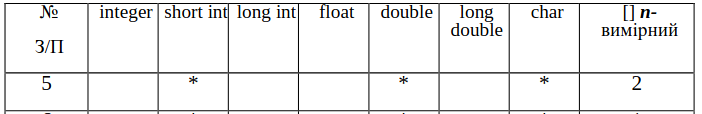
\includegraphics[width=.9\textwidth]{\reportDirectory/var.png}
    \caption{Завдання за варіантом (\variant)}
    \label{fig:task}
\end{figure}


\section{Хід виконання}
Для виконання завдання було обрано мову Rust.
Увесь код також додатково був розміщений в GitHub репозитарії: \href{https://github.com/blackgolyb/algos-labs}{https://github.com/blackgolyb/algos-labs}.


\newpage
\subsection{Підготовка до виконнаня}
Напишемо єдиний інтерфейс для обох таблиць TableMethods.
А також напишемо макрос який буде реалізовувати Display trait для trait TableMethods.

\noindent
Код програми:
\begin{lstlisting}[language=Rust, style=colouredRust]
pub trait TableMethods<T> {
    fn get(&self, i: usize, j: usize) -> T;
    fn set(&mut self, i: usize, j: usize, elem: T);
    fn get_size(&self) -> (usize, usize);
}

#[macro_export]
macro_rules! impl_display_for_table {
    ($table:ident) => {
        impl<T: fmt::Display + Clone> fmt::Display for $table<T> {
            fn fmt(&self, f: &mut fmt::Formatter<'_>) -> fmt::Result {
                let (rows, columns) = self.get_size();
                for i in 0..rows {
                    for j in 0..columns {
                        write!(f, "{} ", self.get(i, j))?;
                    }
                    write!(f, "\n")?;
                }
                Ok(())
            }
        }
    };
}
\end{lstlisting}


\newpage
\subsection{Реалізація стандартної таблиці}
Для реалізації звичайної таблиці зробимо звичайний двовимірний масив який ми заповнюємо коли рядок парний.

\noindent
Код програми:
\begin{lstlisting}[language=Rust, style=colouredRust]
use std::fmt;

use super::base::TableMethods;
use super::impl_display_for_table;

pub struct StandardTable<T> {
    data: Vec<Vec<T>>,
    default_value: T,
    columns: usize,
    rows: usize,
}

impl<T: Clone> TableMethods<T> for StandardTable<T> {
    fn get(&self, i: usize, j: usize) -> T {
        self.data[i][j].clone()
    }

    fn set(&mut self, i: usize, j: usize, elem: T) {
        if i % 2 != 0 {
            self.data[i][j] = self.default_value.clone();
            return;
        }
        self.data[i][j] = elem;
    }

    fn get_size(&self) -> (usize, usize) {
        (self.rows, self.columns)
    }
}

impl<T: Clone> StandardTable<T> {
    pub fn new(rows: usize, columns: usize, default: T) -> Self {
        let mut data: Vec<Vec<T>> = Vec::new();
        for _ in 0..rows {
            data.push(vec![default.clone(); columns]);
        }
        StandardTable {
            data,
            default_value: default.clone(),
            columns,
            rows,
        }
    }
}

impl_display_for_table!(StandardTable);
\end{lstlisting}


\newpage
\subsection{Реалізація економної таблиці}
Для реалізації економної таблиці зробимо одновимірний масив де ми будем зберігати всі елементи.
Для обрахунку індексу такого масиву використаємо функцію $(i / 2) * columns + j$

\noindent
Код програми:
\begin{lstlisting}[language=Rust, style=colouredRust]
use std::fmt;

use super::base::TableMethods;
use super::impl_display_for_table;

pub struct CompactTable<T> {
    data: Vec<T>,
    default_value: T,
    columns: usize,
    rows: usize,
}

impl<T: Clone> TableMethods<T> for CompactTable<T> {
    fn get(&self, i: usize, j: usize) -> T {
        if i % 2 != 0 {
            return self.default_value.clone();
        }
        self.data[(i / 2) * self.columns + j].clone()
    }

    fn set(&mut self, i: usize, j: usize, elem: T) {
        if i % 2 != 0 {
            return;
        }
        self.data[(i / 2) * self.columns + j] = elem;
    }

    fn get_size(&self) -> (usize, usize) {
        (self.rows, self.columns)
    }
}

impl<T: Clone> CompactTable<T> {
    pub fn new(rows: usize, columns: usize, default: T) -> Self {
        CompactTable {
            data: vec![default.clone(); columns * rows.div_ceil(2)],
            default_value: default.clone(),
            columns,
            rows,
        }
    }
}

impl_display_for_table!(CompactTable);
\end{lstlisting}



\newpage
\subsection{Приклад роботи програми}
\noindent
Код програми для перевірки обох таблиць:
\begin{lstlisting}[language=Rust, style=colouredRust]
use std::fmt::Display;
use std::time::Instant;

use super::variants::base::TableMethods;
use super::variants::compact::CompactTable;
use super::variants::standard::StandardTable;

fn table_test<T: TableMethods<i32> + Display>(title: &str, mut table: T) {
    println!("{:=^60}", title);
    let cyles = 1000;
    let (rows, columns) = table.get_size();

    for i in 0..rows {
        for j in 0..columns {
            table.set(i, j, (i + j) as i32);
        }
    }
    println!("{}", table);

    // odd
    let mut read: u128 = 0;
    let mut write: u128 = 0;
    for _ in 0..cyles {
        for i in 0..rows {
            if i % 2 == 0 {
                continue;
            }
            for j in 0..columns {
                let now = Instant::now();
                table.set(i, j, (i + j) as i32);
                write += now.elapsed().as_nanos();
            }
        }
    }
    for _ in 0..cyles {
        for i in 0..rows {
            if i % 2 == 0 {
                continue;
            }
            for j in 0..columns {
                let now = Instant::now();
                table.get(i, j);
                read += now.elapsed().as_nanos();
            }
        }
    }
    println!("Odd rows Times (Read/Write): {} ns / {} ns", read, write);

    // even
    let mut read: u128 = 0;
    let mut write: u128 = 0;
    for _ in 0..cyles {
        for i in 0..rows {
            if i % 2 != 0 {
                continue;
            }
            for j in 0..columns {
                let now = Instant::now();
                table.set(i, j, (i + j) as i32);
                write += now.elapsed().as_nanos();
            }
        }
    }
    for _ in 0..cyles {
        for i in 0..rows {
            if i % 2 != 0 {
                continue;
            }
            for j in 0..columns {
                let now = Instant::now();
                table.get(i, j);
                read += now.elapsed().as_nanos();
            }
        }
    }
    println!("Even rows Times (Read/Write): {} ns / {} ns", read, write);
    println!("{:=^60}\n", "");
}

pub fn main() {
    let rows = 6;
    let columns = 10;

    table_test("Compact Table", CompactTable::<i32>::new(rows, columns, 0));
    table_test(
        "Starndard Table",
        StandardTable::<i32>::new(rows, columns, 0),
    );
}
\end{lstlisting}


\begin{figure}[h!]
    \centering
    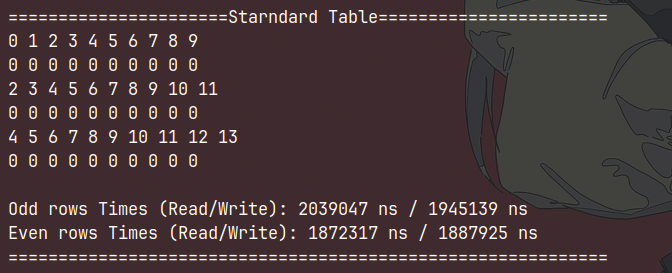
\includegraphics[width=\textwidth]{\reportDirectory/img1.png}
    \caption{Приклад роботи для стандартної таблиці}
    \label{fig:task}
\end{figure}
\begin{figure}[h!]
    \centering
    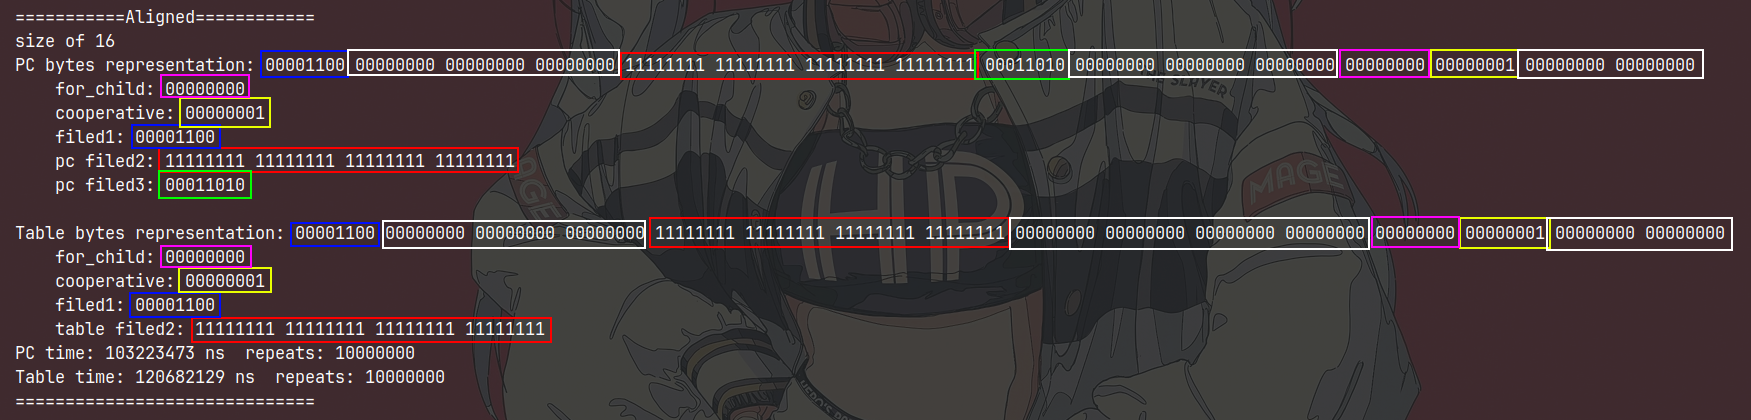
\includegraphics[width=\textwidth]{\reportDirectory/img2.png}
    \caption{Приклад роботи для економної таблиці}
    \label{fig:task}
\end{figure}

\newpage
\section{Висновки}
В ході виконання лабораторної робити було створено стандартну та економну версію таблиць.
Після порівняння швидкодії обох таблиць, компактна таблиця працює швидше,
а особливо швидкість на читання для непарних строк, але й швидкість доступу до парних строк виросла,
бо в нас тільки один рівень вкладеності в масиві.
